\section{Sequentielle Logik}\label{sec:sequentielle-logik}

\subsection{Flip-Flops}\label{subsec:flip-flops}

Ein Flip-Flop ist ein Speicher, der ein Bit speichern, resp.\ festhalten kann.
\begin{center}
    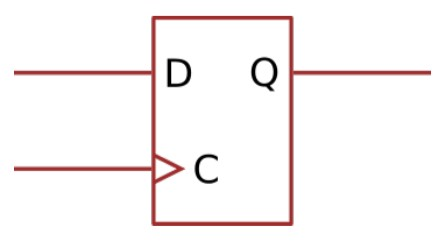
\includegraphics[scale=0.25]{flipflop}
\end{center}
Der Anschluss D ist der Dateneingang, Q der Datenausgang und C ist der Clock-Eingang.
Bei jeder ansteigenden Flanke am Clock-Eingang C übernimmt der Flip-Flop den Zustand vom Eingang D und hält ihn am Ausgang Q fest, bis der Clock eine erneute ansteigende Flanke erhält.

Ein einzelner Flip-Flop kann zwei Zustände speichern, während zwei Flip-Flops vier Zustände speichern können.
Daraus lässt sich ableiten, dass $n$ Flip-Flops $2^n$ Zustände annehmen können.

\subsection{Finite State Machine}\label{subsec:finite-state-machine}

Eine Finite-State-Machine ist eine Schaltung, die Speicher enthält und eine endliche Anzahl von Zustände annehmen kann (daher der Name).
Das Ausgangssignal ist abhängig vom aktuellen Zustand und den Eingangssignalen.
\begin{center}
    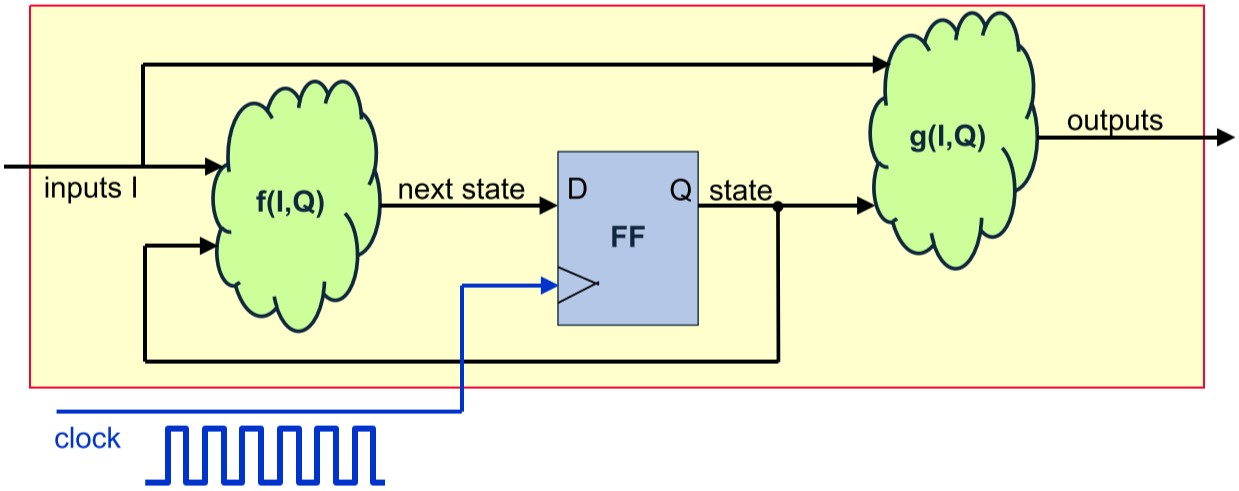
\includegraphics[scale=0.3]{finite-state-machine}
\end{center}
Der $FF$-Block stellt einen Flip-Flop dar und entspricht dem Zustand des Automaten.
Bei jedem Takt-Signal (Clock) wird der Speicher neu geladen.

\subsection{Shiftregister}\label{subsec:register}

Ein Shiftregister (dt.\ Schieberegister) ist eine Schaltung, die mehrere in Reihe geschaltete Flip-Flops enthält.
Bei jedem Signaltakt verschiebt sich der Speicherinhalt der Flip-Flops um eine Position weiter.
Die Anzahl der im Register vorhandenen Speicherplätze ist konstant.
Schieberegister arbeiten nach dem FIFO-Prinzip (First In - First Out), d.h.\ das zuerst eingespeicherte Bit verlässt den Speicher wieder zuerst.
\begin{center}
    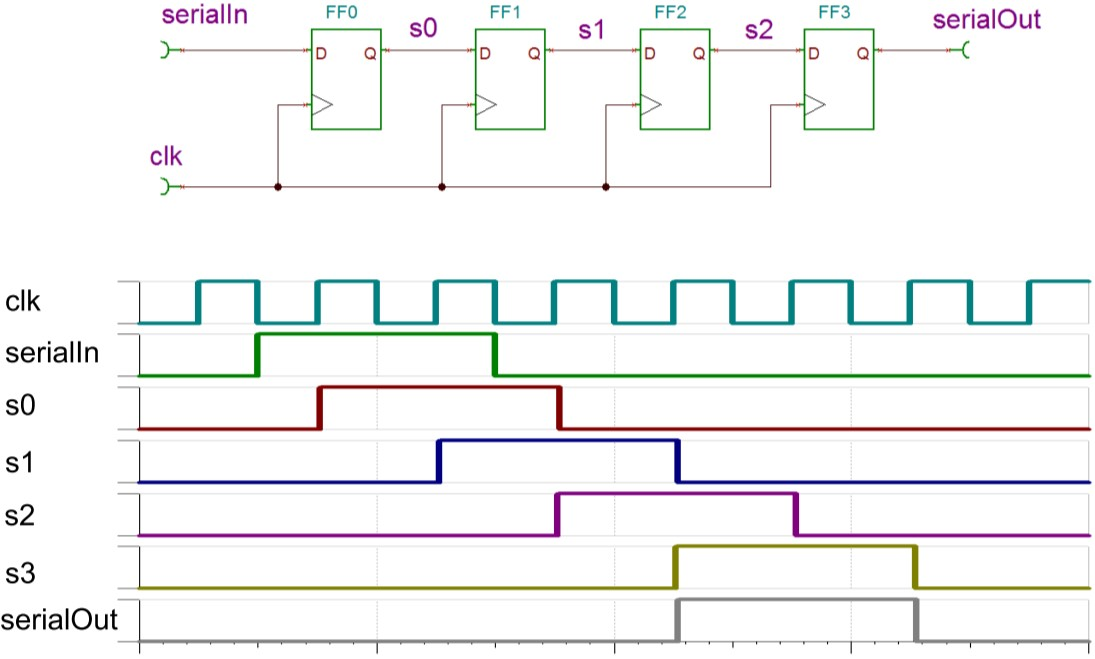
\includegraphics[scale=0.3]{shiftregister-timing-diagram}
\end{center}